\documentclass{article}
\usepackage{graphicx}
\usepackage{multicol} % use to multiple column in itemize
\usepackage{float}
\usepackage{setspace}
\usepackage{hyperref}
\setlength{\parskip}{0.5em}

\begin{document}

\title{Features Premiere}
% \author{Cong Cuong PHAM}

\maketitle

\begin{abstract}
This document introduces some fundamental notions of Features Premiere.
\end{abstract}

\subsection{Features premiere}
\par With enough good data, it's simply amazing what you can get a computer to do. Part of having good data is ensuring your data is organized so it can be processed. To be usable by SciKit-Learn, the machine learning library for Python you'll be using in this course, your data needs to be organized into matrix of {\bf{samples}} and {\bf{features}}.

\begin{figure}[H]
\centering
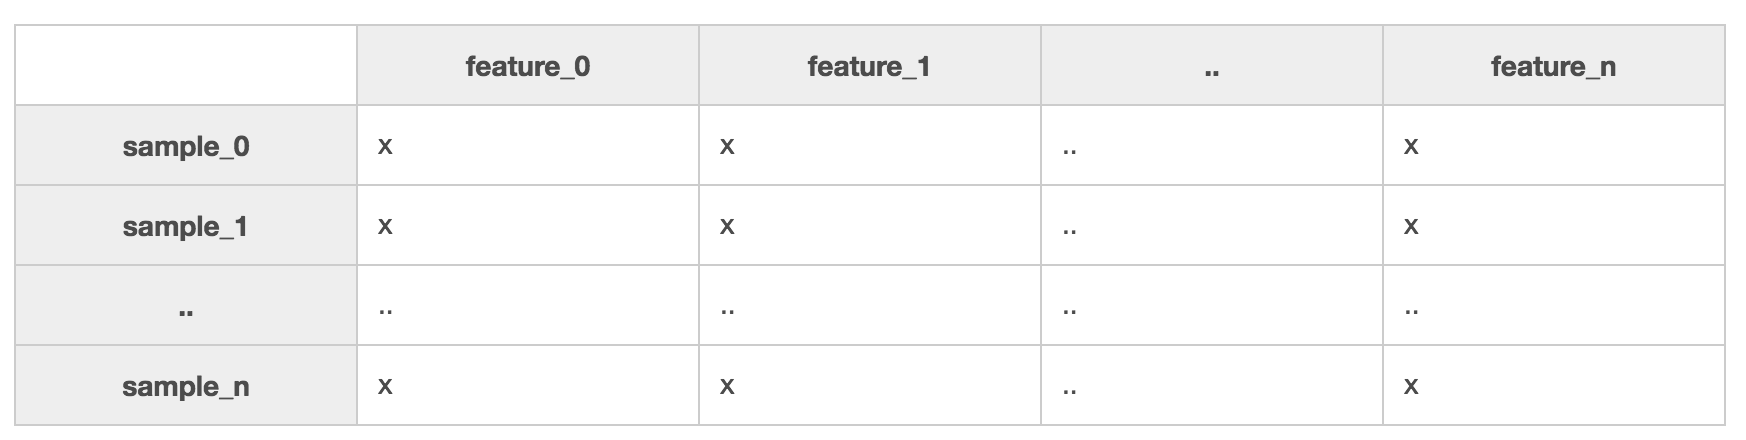
\includegraphics[width=\linewidth]{pic/features-premiere-1.png}
\end{figure}

A sample is any phenomenon you can describe with quantitative traits. They are represented in your dataset by rows. If you were building a dataset of `companies', each sample would be details about a company. When it's said that you need a lot of {\it{data}}, what is generally meant is that you need {\it{many samples}}.

Features are those quantitative traits that describe your samples. They might be {\it{numeric}} or {\it{textual}}, for example, {\it{CompanyName}} is a textual feature in your `companies' dataset. Different samples might result in values such as `Microsoft', `EdX', or `Coding Dojo' for the CompanyName feature. If {\it{CompanyRating}} were a numeric feature in the same dataset, its value might have score between 1 and 5 for each company:

\begin{figure}[H]
\centering
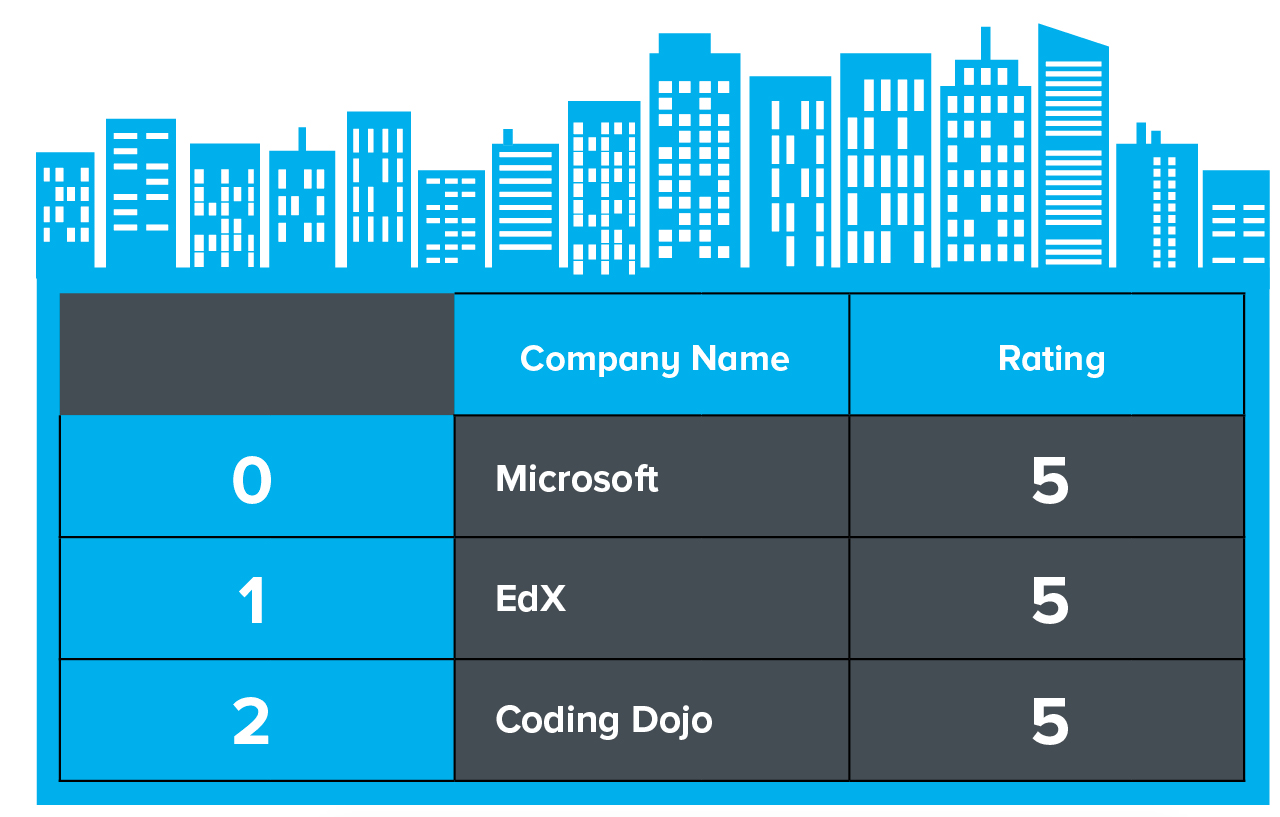
\includegraphics[width=0.8\linewidth]{pic/features-premiere-2.png}
\end{figure}

There are many synonymous names for features. The background of the speaker, as well as the context of the conversation usually dictates which term is used:

\begin{itemize}
	\item {\it{Attribute}} - Features are a quantitative attributes of the samples being observed
	\item {\it{Axis}} - Features are orthogonal axes of their feature space, if they are linearly independent
	\item {\it{Column}} - Features are represented as columns in your dataset
	\item {\it{Dimension}} - A dataset's features, grouped together can be treated as a n-dimensional coordinate space
	\item {\it{Input}} - Feature values are the input of data-driven, machine learning algorithms
	\item {\it{Predictor}} - Features used to predict other attributes are called predictors
	\item {\it{View}} - Each feature conveys a quantitative trait or perspective about the sample being observed
	\item {\it{Independent Variable}} - Autonomous features used to calculate others are like independent variables in algebraic equations
\end{itemize}

Although they have many names, any given feature will fall into one of two types:
\begin{figure}[H]
\centering
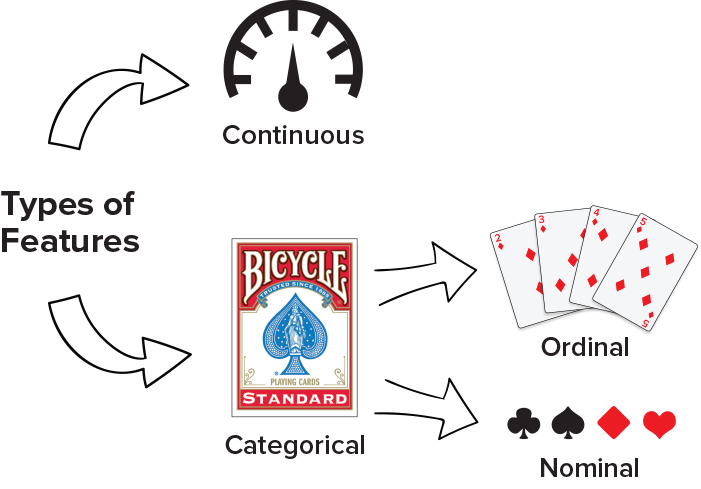
\includegraphics[width=0.8\linewidth]{pic/features-premiere-3.png}
\end{figure}

{\bf{Continuous Features:}}

\par In the case of continuous features, there exist a measurable difference between possible feature values. Feature values usually are also a subset of all real numbers:

\begin{itemize}
	\item Distance
	\item Time
	\item Cost
	\item Temperature
\end{itemize}

{\bf{Categorical Features}}

With categorical features, there is a specified number of discrete, possible feature values. These values may or may not have ordering to them. If they do have a natural ordering, they are called ordinal categorical features. Otherwise if there is no intrinsic ordering, they are called nominal categorical features.

\begin{itemize}
	\item Nominal
		\begin{itemize}
			\item Car Models
			\item Colors
			\item TV Shows
			\item Ordinal
		\end{itemize}
	\item Ordinal		
		\begin{itemize}
			\item High-Medium-Low
			\item 1-10 Years Old, 11-20 Years Old, 30-40 Years Old
			\item Happy, Neutral, Sad
		\end{itemize}
\end{itemize}

{\bf{An Important Note}}

Continuous data is almost always represented with numeric features. But just because you have a numeric feature doesn't cause it to be continuous. There are times where you might have {\it{numerical categorical}} data.

Imagine grading project submissions from groups of students. Each student might individually be assigned a score: 1, 2, 3, where the score represents the group they placed in (first, second, and third place). In this case, you are using a numeric feature to model an ordinal category. However in another dataset, 1, 2, 3 might be used to model nominal data. For example, if you have three different species labeled 1, 2, 3, that labeling has no intrinsic ordering and is thus a nominal category. In these two examples, the ``
numeric" feature represents either ordinal or nominal categorical data.

This is an area that causes confusion for students. What happens if your dataset holds the age of 1000 people recorded in years? Should you treat it as continuous or as ordinal? Though technically ordinal, you can really represent it as either. Your choice should be driven by your {\it{desired outcome}}. If your interests lies in creating a formula that smoothly relates age to other features, treating it as continuous is more correct, even though you were given age-data in intervals. However if you're interested in getting back integer values for age given the other features, treat it as categorical.
  
\begin{flushright}
    source: \href{https://courses.edx.org/courses/course-v1:Microsoft+DAT210x+6T2016/courseware/12621a4064aa4d92874a9d8a953734c5/dfc5af6b20e548b4a62b59b73d71d9bd/}{course.edx.org}  
\end{flushright}

\end{document}